\documentclass[a4paper,12pt]{article}
\usepackage{fontspec}
\usepackage{xeCJK}
\usepackage{graphicx}
\usepackage{float}
\usepackage{hyperref}
\usepackage{listings}
\usepackage{xcolor}
\usepackage{geometry}
\usepackage{titlesec}
\usepackage{booktabs}
\usepackage{caption}
\usepackage{subcaption}
\usepackage{tikz}
\usetikzlibrary{arrows.meta,positioning,fit,calc,backgrounds}

\geometry{left=2.5cm,right=2.5cm,top=2.5cm,bottom=2.5cm}

\providecommand{\mvpRoot}{.}
\IfFileExists{./experiment_results/real_throughput_comparison.pdf}{
  \renewcommand{\mvpRoot}{.}
}{
  \IfFileExists{./legacy/mvp_core/experiment_results/real_throughput_comparison.pdf}{
    \renewcommand{\mvpRoot}{./legacy/mvp_core}
  }{}
}

% Code listing style
\definecolor{codegreen}{rgb}{0,0.6,0}
\definecolor{codegray}{rgb}{0.5,0.5,0.5}
\definecolor{codepurple}{rgb}{0.58,0,0.82}
\definecolor{backcolour}{rgb}{0.95,0.95,0.92}

\lstdefinestyle{mystyle}{
    backgroundcolor=\color{backcolour},
    commentstyle=\color{codegreen},
    keywordstyle=\color{magenta},
    numberstyle=\tiny\color{codegray},
    stringstyle=\color{codepurple},
    basicstyle=\ttfamily\footnotesize,
    breakatwhitespace=false,
    breaklines=true,
    captionpos=b,
    keepspaces=true,
    numbers=left,
    numbersep=5pt,
    showspaces=false,
    showstringspaces=false,
    showtabs=false,
    tabsize=2,
    extendedchars=false % Allow xeCJK to handle Chinese characters
}
\lstset{style=mystyle}

\IfFontExistsTF{Microsoft YaHei}{
    \setCJKmainfont[BoldFont=SimHei, ItalicFont=KaiTi]{Microsoft YaHei}
}{
    \IfFontExistsTF{Noto Sans CJK SC}{\setCJKmainfont{Noto Sans CJK SC}}{\setCJKmainfont{SimSun}}
}

\IfFontExistsTF{SimHei}{
    \setCJKsansfont{SimHei}
}{
    \IfFontExistsTF{Noto Sans CJK SC}{\setCJKsansfont{Noto Sans CJK SC}}{\setCJKsansfont{SimSun}}
}

\IfFontExistsTF{KaiTi}{
    \setCJKmonofont{KaiTi}
}{
    \IfFontExistsTF{Noto Sans Mono CJK SC}{\setCJKmonofont{Noto Sans Mono CJK SC}}{\setCJKmonofont{SimSun}}
}
\XeTeXlinebreaklocale "zh"
\XeTeXlinebreakskip = 0pt plus 1pt

\title{\textbf{系统架构与性能工程报告}\\ \large xy-core 混合调度架构实现细节与实验分析}
\author{Leslie Qi}
\date{2025年12月23日}

\begin{document}

\sloppy
\setlength{\emergencystretch}{2em}

\maketitle

\tableofcontents
\clearpage

\section{工程概述 (Engineering Overview)}

本报告作为核心研究论文的工程补充，聚焦 \textbf{xy-core} 在边缘计算环境下的实现细节、系统架构与可复现实验结果。研究问题定义为：在高并发多模态混合负载（LLM 推理 + 视觉理解 + 图像生成 + 语音合成）下，Python 控制面容易因 GIL 争用、计算密集型负载与外部 I/O 抖动而出现事件循环响应性下降，从而引发端到端尾延迟放大与流式协议不稳定。

为应对上述问题，我们将调度体系组织为 \textbf{Two-Tier Hybrid Architecture (Control Plane vs Data Plane)}：控制平面负责编排、路由、背压与故障处理；数据平面承载计算密集型任务，并尽可能在解释器 GIL 之外执行，以降低控制平面阻塞并增强资源隔离与可预测性。

\section{系统架构实现 (System Architecture Implementation)}

系统采用分层架构设计，以 FastAPI 作为接入层，通过依赖注入容器（\texttt{shared.di}）管理适配器与服务，并使用全局任务调度器（\texttt{GlobalTaskScheduler}）承接需要卸载的计算任务。在调度层面，我们将系统划分为 \textbf{控制平面 (Control Plane)} 与 \textbf{数据平面 (Data Plane)}：

\begin{itemize}
    \item \textbf{Control Plane（L1 Router）}: 运行于主 \texttt{asyncio} 事件循环，负责任务编排、策略驱动路由、失败隔离与降级。该层不直接执行计算密集型任务，而是将负载分发至合适的执行层。
    \item \textbf{Data Plane（L2 Compute）}: 承载计算密集型任务的执行层。在 Two-Tier Hybrid Architecture 中，C++ 调度引擎作为主要的 L2 Compute 节点，将计算从 Python 解释器执行路径中剥离，降低 GIL 争用与事件循环阻塞；当 C++ 调度器不可用或策略不匹配时，自动回退到 Python Worker 作为故障回退（fallback）执行路径。
\end{itemize}

\subsection{架构图与数据流}

系统架构由以下核心组件定义：

\begin{itemize}
    \item \textbf{FastAPI WebSocket Handler}: 负责连接管理、协议封装与流式输出（\texttt{acknowledged/response/response\_done}）。
    \item \textbf{Service Layer (ChatService)}: 封装对话业务流程与流式输出，将底层模型调用抽象为接口（\texttt{LLMInterface/MemoryInterface/ImageGenInterface}）。
    \item \textbf{DI Container (shared.di)}: 管理适配器实例的注册与解析，作为 MVP 的轻量依赖注入机制。
    \item \textbf{全局任务调度器 (GlobalTaskScheduler)}: 作为 \textbf{L1 Control Plane Router} 的统一入口，运行在主 \texttt{asyncio} 事件循环上，为 CPU/GPU 密集型任务提供线程卸载与互斥，并在配置允许时启动/路由到 C++ 引擎。其核心能力包括：
    \begin{itemize}
        \item 任务类型划分：默认异步任务、CPU 绑定任务（CPU-bound）、GPU 绑定任务（GPU-bound）
        \item 任务优先级管理：低、中、高、关键四个优先级
        \item 任务队列：基于优先级的任务队列，支持任务取消和状态管理
        \item Worker 管理：CPU 线程池与 GPU 互斥锁机制
        \item 路由与降级：配置驱动的 A/B 路由，支持按任务类型选择 Python Worker 或 C++ 调度器；失败时自动回退
    \end{itemize}
    \item \textbf{L2 C++ Scheduler Engine}: 通过 pybind11 与 L1 Router 交互，在 Python 解释器全局解释器锁（GIL）临界路径之外执行 LLM 推理与图像生成等计算密集型负载，并提供资源隔离与任务队列管理能力。
    \item \textbf{Python Data Plane (PythonWorker/ThreadPool)}: 作为默认卸载执行层，对 CPU-bound 与 GPU-bound 任务进行线程池卸载，并通过互斥锁避免重型任务并发争抢资源。
    \item \textbf{ResourceManager}: 在 LLM/VL/SD 等重型任务之间执行互斥卸载，降低显存压力并避免 OOM。
\end{itemize}

\begin{figure}[H]
    \centering
    \resizebox{0.98\linewidth}{!}{%
    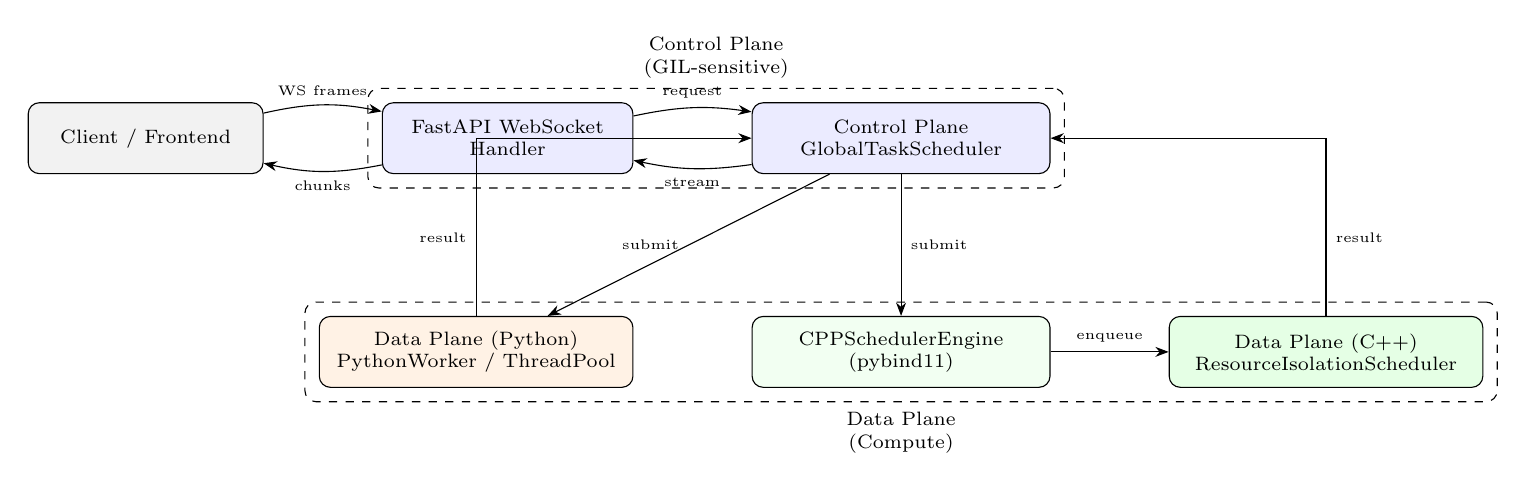
\begin{tikzpicture}[
        font=\scriptsize,
        >=Stealth,
        node distance=18mm,
        box/.style={draw, rounded corners, minimum height=9mm, align=center, inner sep=2.6pt, text width=30mm},
        cbox/.style={box, fill=blue!8, text width=30mm},
        dbox/.style={box, fill=green!10, text width=38mm},
        pbox/.style={box, fill=orange!10, text width=38mm}
    ]
        \node[box, fill=gray!10, text width=28mm] (client) {Client / Frontend};
        \node[cbox, right=15mm of client] (ws) {FastAPI WebSocket\\Handler};
        \node[cbox, right=15mm of ws, text width=36mm] (router) {Control Plane\\GlobalTaskScheduler};

        \node[box, fill=green!5, below=18mm of router, text width=36mm] (binding) {CPPSchedulerEngine\\(pybind11)};
        \node[dbox, right=15mm of binding] (cpp) {Data Plane (C++)\\ResourceIsolationScheduler};
        \node[pbox, left=15mm of binding] (py) {Data Plane (Python)\\PythonWorker / ThreadPool};

        \draw[->] (client) to[bend left=12] node[above, font=\tiny]{WS frames} (ws);
        \draw[->] (ws) to[bend left=12] node[below, font=\tiny]{chunks} (client);

        \draw[->] (ws) to[bend left=10] node[above, font=\tiny]{request} (router);
        \draw[->] (router) -- node[left, font=\tiny]{submit} (py);
        \draw[->] (router) -- node[right, font=\tiny]{submit} (binding);
        \draw[->] (binding) -- node[above, font=\tiny]{enqueue} (cpp);
        \draw[->] (py) |- node[pos=0.22,left, font=\tiny]{result} (router);
        \draw[->] (cpp) |- node[pos=0.22,right, font=\tiny]{result} (router);
        \draw[->] (router) to[bend left=10] node[below, font=\tiny]{stream} (ws);

        \begin{pgfonlayer}{background}
            \node[draw, dashed, rounded corners, inner sep=5pt, fit=(ws) (router), label={[font=\scriptsize]above:{\shortstack{Control Plane\\(GIL-sensitive)}}}] (cpfit) {};
            \node[draw, dashed, rounded corners, inner sep=5pt, fit=(py) (binding) (cpp), label={[font=\scriptsize]below:{\shortstack{Data Plane\\(Compute)}}}] (dpfit) {};
        \end{pgfonlayer}
    \end{tikzpicture}%
    }
    \caption{Two-Tier 混合调度拓扑（Control Plane vs Data Plane）。控制平面在主事件循环中完成编排与路由；数据平面承载计算密集型负载，并通过 C++ 调度器或 Python Worker 执行。}
\end{figure}

数据流流程：
\begin{enumerate}
    \item 请求通过 WebSocket 进入系统，由 WebSocket Handler 解析并生成 \texttt{request\_id}。
    \item Handler 立即发送 \texttt{acknowledged}，随后调用 \texttt{ChatService} 进入流式业务流程。
    \item \texttt{ChatService} 基于容器解析出的 \texttt{LLMInterface} 进行流式生成，并逐 chunk 输出 \texttt{response}。
    \item 当输出包含 \texttt{[GEN\_IMG: ...]} 时，Handler 触发 \texttt{image\_trigger}，并将图像任务进入有界队列以实现背压。
    \item 对需要卸载的计算任务，由 \texttt{GlobalTaskScheduler} 将任务分发到 PythonWorker（线程池卸载）或 C++ Scheduler Engine（可选）。
    \item 无论成功或异常，Handler 都发送 \texttt{response\_done} 结束该请求的流式生命周期。
\end{enumerate}

\begin{figure}[H]
    \centering
    \resizebox{0.98\linewidth}{!}{%
    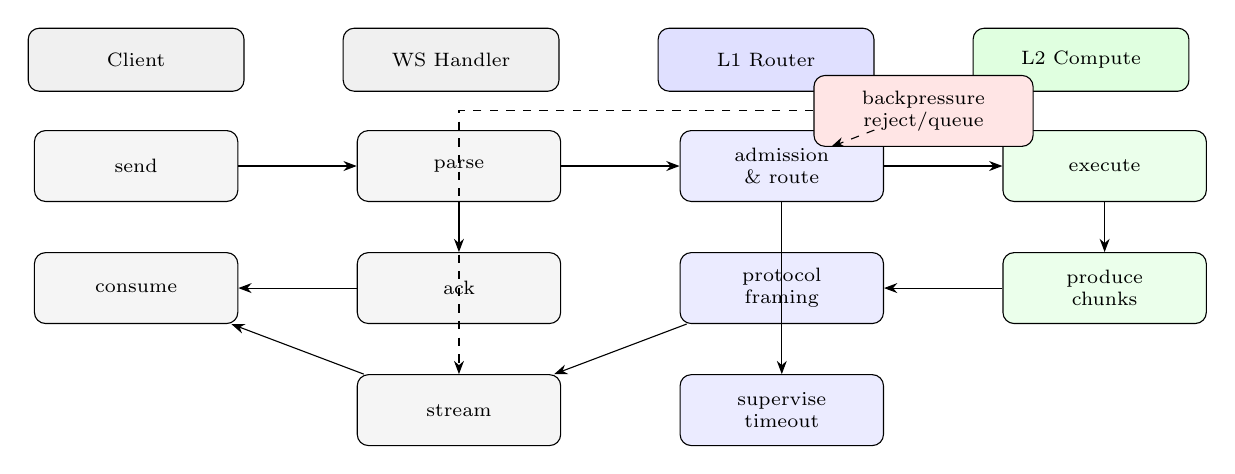
\begin{tikzpicture}[
        font=\scriptsize,
        >=Stealth,
        box/.style={draw, rounded corners, minimum height=9mm, align=center, fill=gray!8, inner sep=2.6pt, text width=24mm},
        lane/.style={draw, rounded corners, minimum height=8mm, align=center, fill=gray!12, inner sep=2pt, text width=26mm}
    ]
        \node[lane] (l1) at (0, 0) {Client};
        \node[lane] (l2) at (4.0, 0) {WS Handler};
        \node[lane, fill=blue!12] (l3) at (8.0, 0) {L1 Router};
        \node[lane, fill=green!12] (l4) at (12.0, 0) {L2 Compute};

        \node[box] (c1) at (0, -1.35) {send};
        \node[box] (w1) at (4.1, -1.35) {parse};
        \node[box, fill=blue!8] (r1) at (8.2, -1.35) {admission\\\& route};
        \node[box, fill=green!8] (d1) at (12.3, -1.35) {execute};

        \node[box] (w2) at (4.1, -2.9) {ack};
        \node[box, fill=blue!8] (r3) at (8.2, -2.9) {protocol\\framing};
        \node[box, fill=green!8] (d2) at (12.3, -2.9) {produce\\chunks};
        \node[box] (c2) at (0, -2.9) {consume};
        \node[box] (w3) at (4.1, -4.45) {stream};
        \node[box, fill=blue!8] (r2) at (8.2, -4.45) {supervise\\timeout};

        \draw[->] (c1) -- (w1);
        \draw[->] (w1) -- (r1);
        \draw[->] (r1) -- (d1);
        \draw[->] (d1) -- (d2);
        \draw[->] (d2) -- (r3);
        \draw[->] (r3) -- (w3);
        \draw[->] (w3) -- (c2);
        \draw[->] (w1) -- (w2);
        \draw[->] (w2) -- (c2);
        \draw[->] (r1) -- (r2);

        % Move backpressure box to not overlap with lanes if it was, but here coordinates look okay.
        % Just ensure it is drawn on top or separate.
        \node[box, fill=red!10, text width=26mm] (bp) at (10.0, -0.65) {backpressure\\reject/queue};
        \draw[->, dashed] (r1) -- (bp);
        % Route dashed line around other boxes if needed, or straight
        \draw[->, dashed] (bp) -| (w3);
    \end{tikzpicture}%
    }
    \caption{请求处理泳道图（含背压）。控制平面完成准入控制、路由与协议封装；数据平面执行计算密集型负载并产出增量结果；当队列容量受限时，控制平面触发背压并以协议化错误/延迟策略维持稳定性。}
\end{figure}

\subsection{资源划分策略}

\begin{table}[H]
\centering
\begin{tabular}{lll}
\toprule
\textbf{资源类型} & \textbf{分配任务} & \textbf{隔离机制} \\
\midrule
\textbf{CPU (主线程)} & WebSocket Handler、ChatService、任务调度器 & Asyncio 协程 \\
\textbf{CPU (线程池)} & CPU 绑定任务（CPU-bound）、模块初始化、业务逻辑 & ThreadPoolExecutor \\
\textbf{GPU} & LLM 推理、VL 视觉理解、图像生成 & 异步互斥与队列化执行 \\
\textbf{内存} & 模型加载、任务数据、缓存 & 模块级内存管理 \\
\bottomrule
\end{tabular}
\caption{资源划分与隔离策略}
\end{table}

\section{工程实现细节 (Engineering Implementation Details)}

\subsection{Worker 协程实现}
系统采用基于协程的 Worker 模型，由 GlobalTaskScheduler 管理多个 Worker 协程，负责从任务队列中获取并执行任务。Worker 协程数量在启动时由配置确定，运行过程中保持固定（当前未实现自动弹性伸缩），但调度器会定期清理已完成任务以释放资源。

Worker 实现特点：
\begin{itemize}
    \item 基于协程的轻量级设计，减少调度开销。
    \item 支持任务优先级与类型划分（默认/CPU-bound/GPU-bound）。
    \item 内置任务状态管理与容错机制（失败标记、异常捕获、Future 完成通知）。
    \item 定期清理已完成任务，释放资源。
\end{itemize}

\begin{lstlisting}[language=Python, caption=Worker 协程实现]
async def _worker_coroutine(self, worker_name: str):
    """
    工作协程，负责从队列中获取任务并执行
    Args:
        worker_name: 工作协程名称
    """
    logger.debug(f"工作协程 {worker_name} 已启动")
    try:
        while self._running:
            task_info = None
            try:
                _, task_info = await asyncio.wait_for(self._task_queue.get(), timeout=1.0)

                if task_info.cancel_requested:
                    logger.debug(f"任务 {task_info.task_id} 已被取消，跳过执行")
                    task_info.status = TaskStatus.CANCELLED
                    continue

                logger.debug(
                    f"工作协程 {worker_name} 开始执行任务 {task_info.task_id} ({task_info.task_type.value})"
                )

                async with self._lock:
                    task_info.status = TaskStatus.RUNNING
                    task_info.start_time = time.time()

                result = await self._execute_task(
                    task_func, task_info.task_type, *task_args, **task_kwargs
                )

                async with self._lock:
                    task_info.status = TaskStatus.COMPLETED
                    task_info.result = result
                    task_info.end_time = time.time()

                logger.debug(f"任务 {task_info.task_id} 执行成功")
            except asyncio.TimeoutError:
                continue
            except Exception as e:
                async with self._lock:
                    if task_info is not None:
                        task_info.status = TaskStatus.FAILED
                        task_info.error = str(e)
                        task_info.end_time = time.time()

                if task_info is not None:
                    logger.error(f"任务 {task_info.task_id} 执行失败: {str(e)}", exc_info=True)
            finally:
                if task_info is not None:
                    self._task_queue.task_done()
    except Exception as e:
        logger.error(f"工作协程 {worker_name} 发生错误: {str(e)}", exc_info=True)
    finally:
        logger.debug(f"工作协程 {worker_name} 已停止")
\end{lstlisting}

\subsection{Scheduler 事件模型}
全局任务调度器 (GlobalTaskScheduler) 采用非阻塞事件驱动设计，支持多种任务类型和优先级。调度器主要功能包括：

\begin{itemize}
    \item 任务调度与执行
    \item 任务优先级管理
    \item 任务状态跟踪
    \item 任务清理机制
\end{itemize}

\begin{lstlisting}[language=Python, caption=任务调度逻辑]
async def schedule_task(
    self,
    func: Callable,
    name: str = "unnamed_task",
    priority: Union[TaskPriority, int] = TaskPriority.MEDIUM,
    task_type: TaskType = TaskType.DEFAULT,
    args: tuple = (),
    kwargs: dict = None
) -> str:
    """
    调度一个新任务
    Args:
        func: 要执行的函数
        name: 任务名称
        priority: 任务优先级
        task_type: 任务类型 (DEFAULT, CPU_BOUND, GPU_BOUND)
        args: 函数位置参数
        kwargs: 函数关键字参数
    Returns:
        任务ID
    """
    if not self._running:
        raise RuntimeError("调度器未启动")
        
    # 创建任务信息
    task_id = f"task_{uuid.uuid4().hex[:8]}_{self._next_task_id}"
    self._next_task_id += 1
    
    task_info = TaskInfo(
        task_id=task_id,
        name=name,
        priority=priority,
        task_type=task_type,
        created_at=time.time(),
        status=TaskStatus.PENDING
    )
    
    # 存储任务信息
    async with self._lock:
        self._tasks[task_id] = {
            'info': task_info,
            'func': func,
            'args': args,
            'kwargs': kwargs
        }
        loop = asyncio.get_running_loop()
        self._task_futures[task_id] = loop.create_future()
        
    # 将任务放入优先级队列
    await self._task_queue.put((-priority.value, task_info))
    
    logger.debug(f"任务已调度 - ID: {task_id}, 名称: {name}, 优先级: {priority.name}, 类型: {task_type.name}")
    return task_id
\end{lstlisting}

\subsection{LLM Worker 通信与容错}
主调度器与功能模块之间通过异步方式通信，支持任务结果的异步获取。系统内置了完善的容错机制：

\begin{itemize}
    \item \textbf{任务执行容错}: 任务执行失败时，自动更新任务状态并记录错误信息
    \item \textbf{异步异常处理}: 使用 asyncio.Future 处理异步任务异常
    \item \textbf{资源自动释放}: 任务完成后自动释放相关资源
    \item \textbf{取消与中止}: 任务可被标记为取消并在 Worker 获取时跳过执行
\end{itemize}

\begin{lstlisting}[language=Python, caption=任务容错处理]
# 执行任务
try:
    result = await self._execute_task(
        task_func, task_info.task_type, *task_args, **task_kwargs
    )
    
    # 更新任务状态为完成
    async with self._lock:
        task_info.status = TaskStatus.COMPLETED
        task_info.result = result
        task_info.end_time = time.time()
        
        fut = self._task_futures.get(task_info.task_id)
        if fut and not fut.done():
            fut.set_result(result)
            
except Exception as e:
    # 更新任务状态为失败
    async with self._lock:
        task_info.status = TaskStatus.FAILED
        task_info.error = str(e)
        task_info.end_time = time.time()
        
        fut = self._task_futures.get(task_info.task_id)
        if fut and not fut.done():
            fut.set_exception(e)
            
    logger.error(f"任务 {task_info.task_id} 执行失败: {str(e)}", exc_info=True)
\end{lstlisting}

\section{功能模块描述 (Function Module Description)}

系统采用分层的服务化设计：接入层由 FastAPI WebSocket Handler 负责协议与连接管理；业务层由 \texttt{ChatService} 组织对话流程并以流式事件输出；基础设施层通过 \texttt{shared.di} 进行适配器注册与解析。模块间的“事件”以 \texttt{async generator} 产生的结构化消息在调用链中向上传递，并由 Handler 统一封装为 WebSocket 帧。

\subsection{Service Container \& Dependency Injection}

系统采用基于 FastAPI 的轻量级服务架构，通过依赖注入 (Dependency Injection) 容器管理组件生命周期。

\subsubsection{架构设计}
\begin{itemize}
    \item \textbf{DI Container}: 使用 \texttt{shared.di} 容器统一管理单例服务（LLM, Memory, ImageGen）。
    \item \textbf{Service Layer}: \texttt{ChatService} 封装核心业务逻辑，协调各适配器。
    \item \textbf{Adapter Pattern}: 所有外部模型（LLM, SD, TTS）均通过标准接口（Adapter）接入，屏蔽具体实现差异。
\end{itemize}

\begin{lstlisting}[language=Python, caption=依赖注入与服务启动 (main.py)]
def bootstrap():
    # Register Dependencies
    settings = get_settings()
    
    # LLM Adapter Registration
    if os.path.exists(settings.model.text_path):
        container.register(
            LLMInterface,
            GGUFLLMAdapter(...)
        )
    else:
        container.register(LLMInterface, MockLLMAdapter())

    # Image Generation Adapter
    container.register(ImageGenInterface, SDAdapter(sd_conf))
    
    # Initialize Character
    aveline = CharacterProfile(name="Aveline", ...)
    return aveline

app = FastAPI()
character = bootstrap()
chat_service = ChatService(character)
ws_handler = WebSocketHandler(chat_service)
\end{lstlisting}

\subsection{任务调度器模块 (GlobalTaskScheduler)}

GlobalTaskScheduler 是系统的任务管理核心，负责调度和执行所有类型的任务。

\subsubsection{功能与架构}
\begin{itemize}
    \item 支持多种任务类型：默认异步任务、CPU 密集型任务、GPU 密集型任务。
    \item 支持任务优先级管理：低、中、高、关键四个优先级。
    \item 支持任务状态跟踪和管理（创建/运行/完成/失败/取消）。
    \item 支持任务清理和资源释放（定期清理已完成任务记录）。
\end{itemize}

\subsubsection{任务管理机制}

任务调度器实现了完整的任务生命周期管理（当前版本不包含独立的“周期性任务调度器”，周期性/定时行为可由上层业务通过显式提交任务实现）：

\begin{enumerate}
    \item \textbf{任务创建}: 根据任务类型和优先级创建任务
    \item \textbf{任务调度}: 将任务放入优先级队列等待执行
    \item \textbf{任务执行}: Worker 协程从队列中获取任务并执行
    \item \textbf{任务状态更新}: 实时更新任务状态
    \item \textbf{任务结果返回}: 将任务结果返回给请求方
    \item \textbf{任务清理}: 定期清理已完成的旧任务
\end{enumerate}

\subsection{其他功能模块}

\subsubsection{LLM模块}
负责大语言模型的推理和生成，支持多种模型和推理框架。

\subsubsection{视觉理解模块 (Visual Understanding Module)}
负责图像内容的深度理解与分析，基于 Qwen2-VL 模型。支持视觉问答（VQA）、场景描述生成及图文多模态推理，作为 GPU 密集型任务由调度器统一管理。

\subsubsection{图像生成模块 (Image Generation Module)}
负责创意图像生成，基于 Stable Diffusion 1.5 的文生图（Text-to-Image）链路。在 MVP 基准中不引入独立的图生图接口，重点验证生成卸载、资源互斥与背压控制等工程约束。

\subsubsection{语音模块}
负责语音合成（TTS）能力。基准脚本可加载 GPT-SoVITS 适配器作为 CPU/IO 负载注入，用于复现综合多模态压力；MVP WebSocket 交互链路默认不依赖 STT。

\subsubsection{内存模块}
MVP 采用 \texttt{InMemoryMemoryRepository} 作为 \texttt{MemoryInterface} 的实现，提供对话历史追加/读取与简单关键字检索，用于验证接口形态与链路完整性。

\section{最新特性介绍 (Latest Features Introduction)}

\subsection{情感智能 (Emotional Intelligence)}

MVP 形态下系统提供“角色状态”与“触发器”机制，用于在提示词中注入可控的情绪/亲密度上下文，并在命中关键词时产生结构化事件。

\subsubsection{角色状态注入}
\begin{itemize}
    \item \textbf{状态字段}: \texttt{CharacterProfile} 维护 \texttt{current\_emotion} 与 \texttt{intimacy\_level} 等运行时状态。
    \item \textbf{提示词拼接}: \texttt{ChatService} 在构建 \texttt{system\_prompt} 时将状态信息拼接进提示词，影响生成风格。
\end{itemize}

\subsubsection{触发器与事件输出}
\begin{itemize}
    \item \textbf{Sensory Triggers}: 当输入命中预设关键词，\texttt{ChatService} 产出 \texttt{sensory\_trigger} 事件。
    \item \textbf{Behavior Chains}: 当输入命中行为链关键词，\texttt{ChatService} 产出 \texttt{behavior\_chain} 事件。
    \item \textbf{协议承载}: WebSocket Handler 将上述事件统一封装为 \texttt{type=event} 的帧，并携带事件名与数据。
\end{itemize}

\subsection{多模态交互 (Multimodal Interaction)}

系统在 MVP 基准中覆盖多模态链路（文本生成 + 图像生成，并在实验脚本中覆盖 TTS/VL 任务），重点验证“重型任务卸载、背压与可观测性”而非完整的产品级多模态 UI 交互闭环。

\subsubsection{多模态融合处理}
\begin{itemize}
    \item \textbf{文本链路}: \texttt{ChatService} 通过 \texttt{LLMInterface} 流式输出 token。
    \item \textbf{实验链路}: \texttt{comprehensive\_experiment.py} 在 \texttt{real/mock} 模式下加载 VL/TTS 适配器，用于复现边缘设备的综合负载。
\end{itemize}

\subsubsection{多模态输出生成}
\begin{itemize}
    \item \textbf{图像触发}: 当 LLM 输出包含 \texttt{[GEN\_IMG: ...]}，\texttt{ChatService} 产出 \texttt{image\_trigger} 事件。
    \item \textbf{背压队列}: WebSocket Handler 将图像任务进入有界队列，并通过 \texttt{image\_status/image\_error} 回传排队与失败信息。
    \item \textbf{任务执行}: 图像生成由 \texttt{ImageGenInterface} 适配器执行（真实 SDAdapter 或合成适配器）。
\end{itemize}

\subsection{流式事件序列 (Streaming Event Sequence)}

系统在 MVP 中不引入独立事件总线组件，而是采用“生成器事件流 + 协议封装”的方式实现事件驱动：业务层将过程拆解为一系列结构化事件，由接入层统一编码为 WebSocket 帧，从而做到低耦合与可观测。

\subsubsection{事件来源与类型}
\begin{itemize}
    \item \textbf{token}: LLM 流式增量输出。
    \item \textbf{image\_trigger}: 文本中声明式触发图像生成。
    \item \textbf{sensory\_trigger/behavior\_chain}: 关键词触发的结构化事件。
\end{itemize}

\subsubsection{协议化封装}
\begin{itemize}
    \item \textbf{三段式流式协议}: 每次请求固定输出 \texttt{acknowledged} / \texttt{response} / \texttt{response\_done}。
    \item \textbf{事件承载}: 非 token 的事件统一以 \texttt{type=event} 或专用帧（如 \texttt{image\_trigger}）回传。
    \item \textbf{错误分级}: 异常被封装为 \texttt{type=error}，并携带可重试标记与错误类型。
\end{itemize}

\section{新版 MVP 设计目标与基准定义 (MVP v2 Baseline)}

为了将工程能力从论文级验证推进到可持续迭代的主程序，我们在原 MVP 的基础上引入了“可复现实验基准”这一中间层：先在一个可控的最小系统中，把关键链路与约束条件跑通并固化为基准测试，再逐步迁移到主工程。

\subsection{目标与范围}

\begin{itemize}
    \item \textbf{目标}: 构建一个可重复、可对比、可回归的实验基准，用于评估调度、资源互斥、流式协议与多模态链路的稳定性。
    \item \textbf{范围}: 保留 MVP 的模块化与负载注入框架，同时对齐主工程近期新增的能力：严格显存互斥策略、流式协议一致性与图像生成并行事件。
    \item \textbf{非目标}: 不追求 UI/产品完整性；不在基准系统中实现所有业务模块，只覆盖对性能与可靠性最敏感的链路。
\end{itemize}

\subsection{新版 MVP 的最小能力集}

\begin{enumerate}
    \item \textbf{严格互斥的资源治理}: 在 LLM / VL / 图像生成三类重型任务之间实现互斥加载与卸载，确保 8GB/12GB 显存环境可预测运行。
    \item \textbf{流式协议对齐}: WebSocket 统一输出 \texttt{acknowledged} / \texttt{response} / \texttt{response\_done} 三段式消息，保证前端/客户端可进行稳定的流式消费与状态管理。
    \item \textbf{图像并行事件链路}: 当输出包含 \texttt{[GEN\_IMG: ...]} 时产生 \texttt{image\_trigger} 事件，使“边画图边聊天”的状态与结果可被独立观测与回归。
    \item \textbf{双模负载}: 继续保留 \texttt{mock} 与 \texttt{real} 两种模式，用于剥离模型因素并验证真实硬件约束下的长尾行为。
\end{enumerate}

\subsection{基准指标 (Metrics)}

\begin{itemize}
    \item \textbf{吞吐量（Throughput）}: RPS 随并发变化的曲线。
    \item \textbf{端到端延迟}: P50/P95/P99 延迟分位数。
    \item \textbf{主线程阻塞}: Event Loop Lag（监控协程的 sleep 误差）衡量阻塞程度。
    \item \textbf{稳定性}: 固定时间窗口内的完成数与错误数。
    \item \textbf{协议一致性}: 每个请求必须产生完整的 \texttt{acknowledged} 与 \texttt{response\_done}，且中间响应序列可重放。
\end{itemize}

\section{实验环境 (Experiment Environment)}

\subsection{双模验证机制 (Dual-Mode Verification)}

为了确保实验数据的真实性与调度算法的可复现性，本研究设计了两种实验基准：

\begin{itemize}
    \item \textbf{全真实边缘负载 (Full Real-World Edge Load)}:

    该模式部署了完整的量化模型矩阵，包括 Qwen2.5-7B-Instruct (Q4\_K\_M) 作为核心推理引擎（本次实验中针对 8GB 显存设备配置为 CPU Offload 模式），Qwen2-VL-2B 处理视觉任务，以及 GPT-SoVITS 与 Stable Diffusion 1.5。

    该模式用于采集第 7 章中所有的真实性能指标（吞吐量、显存占用、延迟）。

    \item \textbf{合成压力负载 (Synthetic Stress Simulation)}:

    为了剥离模型加载时间对调度逻辑分析的干扰，并验证极端条件下的系统稳定性，我们构建了一套“重负载模拟器”。

    该模拟器通过矩阵运算与内存操作，精确复现了真实模型的 CPU 阻塞特征 与 显存瞬时脉冲特征，用于验证第 8 章中的长尾延迟与错误恢复机制。
\end{itemize}

\subsection{边缘约束模拟 (Edge Constraints Simulation)}

实验在模拟边缘设备约束的受控环境中进行。

\begin{itemize}
    \item \textbf{硬件配置}: AMD Ryzen 9 8940HX, NVIDIA RTX 5070 Laptop GPU。
    \item \textbf{模拟约束}:
    \begin{itemize}
        \item \textbf{GPU 功耗限制}: 限制功耗以模拟低功耗边缘 GPU。
        \item \textbf{内存限制}: 系统可用 RAM 限制为 16GB。
        \item \textbf{CPU 核心}: Worker 绑定特定核心，模拟 4 核嵌入式处理器。
    \end{itemize}
    \item \textbf{负载注入}: 使用自定义负载注入器 (\texttt{comprehensive\_experiment.py}) 生成标准化多模态任务链 (Standardized Multimodal Pipeline)，每个任务包含完整的交互流程：
    \begin{itemize}
        \item \textbf{1x LLM 推理} (CPU Offload, Qwen2.5-7B)
        \item \textbf{1x 语音合成} (Network/IO, GPT-SoVITS)
        \item \textbf{1x 视觉理解} (GPU, Qwen2-VL)
        \item \textbf{1x 图像生成} (GPU, Stable Diffusion 1.5)
    \end{itemize}
    \textbf{说明}: 这种“全模态”负载设计旨在模拟最极端的并发场景，测试系统在所有组件同时满载时的调度能力。
\end{itemize}

\section{实验评估 (Experimental Evaluation)}

\subsection{真实负载性能对比 (Real Workload Performance Comparison)}

我们在真实负载模式下，对比了两种运行形态的性能表现：\textbf{xy-core（Python 调度器）}与 \textbf{xy-core（C++ Hybrid 调度器）}。实验负载为标准化多模态任务链（LLM 推理 + TTS 合成 + 视觉理解 + 图像生成）。

\begin{figure}[H]
    \centering
    \includegraphics[width=0.8\linewidth]{\mvpRoot/experiment_results/real_throughput_comparison.pdf}
    \caption{真实负载吞吐量随并发变化（RPS vs Concurrency）。该图对比了 Python 与 C++ Hybrid 的端到端吞吐表现。}
\end{figure}

\begin{figure}[H]
    \centering
    \includegraphics[width=0.8\linewidth]{\mvpRoot/experiment_results/real_latency_percentiles.pdf}
    \caption{真实负载端到端延迟分位数（Exp3，P50/P95/P99）。该图展示在相同请求链路下的延迟分布差异。}
\end{figure}

\begin{figure}[H]
    \centering
    \includegraphics[width=0.8\linewidth]{\mvpRoot/experiment_results/real_event_loop_lag.pdf}
    \caption{真实负载下的控制平面响应性（Exp2，Event Loop Lag）。以监控协程的 sleep 漂移量（sleep drift, ms）近似事件循环延迟，用于刻画在多模态混合负载下控制平面是否出现可观测的阻塞尖峰。}
\end{figure}

\begin{figure}[H]
    \centering
    \includegraphics[width=0.8\linewidth]{\mvpRoot/experiment_results/image_backpressure_real.pdf}
    \caption{图像生成背压（backpressure）微基准（Real）。在有界队列（bounded queue）容量受限时统计接收、拒绝与完成数量，用于验证控制平面的准入控制（admission control）与资源隔离行为。}
\end{figure}

\subsection{硬件遥测与执行轨迹 (NVIDIA-SMI \& Trace)}

为了补齐“可解释的证据链”，我们补充了两类在工业界与学术界常用的可观测性产物：\textbf{GPU 遥测快照（NVIDIA-SMI）}与\textbf{调度执行轨迹（Trace Timeline）}。前者用于展示显存压力（VRAM pressure）与设备利用率（utilization），后者用于展示任务在 Control Plane 与 Data Plane 间的调度序列与执行重叠情况。

\begin{figure}[H]
    \centering
    \includegraphics[width=0.95\linewidth]{\mvpRoot/experiment_results/scheduler_trace_timeline.pdf}
    \caption{调度执行轨迹（逻辑甘特图，log-based）。横轴为时间，纵轴为执行通道；以“排队（scheduled\textrightarrow started）+ 执行（started\textrightarrow completed）”的分段可视化刻画队列时延与执行时长，用于分析路由决策与并行重叠。}
\end{figure}

\input{\mvpRoot/experiment_results/scheduler_trace_index.tex}

\begin{figure}[H]
    \centering
    \includegraphics[width=0.95\linewidth]{\mvpRoot/experiment_results/memory_usage_over_time.pdf}
    \caption{显存占用随时间变化（VRAM Usage over Time）。横轴为时间（秒），纵轴为显存占用（GB）；在曲线上标注了“加载模型”、“生成图像”、“卸载模型”的关键时刻，用于直观展示重型任务对显存压力的动态影响。}
\end{figure}

\subsection{朴素异步基线对比 (Naive Async Baseline, Mock Workload)}

为避免“只与历史版本对比”的叙事偏差，我们引入两类更具解释力的基线：\textbf{朴素异步 (naive async)} 与 \textbf{串行基线 (single thread)}。

\textbf{naive async} 定义为：在同一 \texttt{asyncio} 事件循环中直接执行重型 CPU/GPU 模拟负载，并仅以 \texttt{asyncio.gather} 拉高并发；该范式在吞吐上可能受益于并发发起，但其控制平面将与计算密集型负载竞争时间片，更易出现 event loop starvation。\textbf{xy-core} 的 Two-Tier 设计则将重负载显式卸载到数据平面（线程池或 C++ 调度器），将控制平面约束为“轻量、可预测”的编排路径。

该组对比采用 \textbf{Mock Workload}，以隔离模型体积、网络抖动与外部服务可用性等变量，突出调度架构对吞吐、尾延迟与控制平面响应性的影响（结果文件 \texttt{legacy/mvp\_core/experiment\_results/*\_mock.json}）。

\begin{figure}[H]
    \centering
    \includegraphics[width=0.88\linewidth]{\mvpRoot/experiment_results/mock_exp1_concurrency_rps.pdf}
    \caption{Mock 基线吞吐对比（Exp1）。对比 single thread、naive async 与 xy-core（Python/C++ Image 路由）的并发吞吐表现。}
\end{figure}

\begin{figure}[H]
    \centering
    \includegraphics[width=0.88\linewidth]{\mvpRoot/experiment_results/mock_exp2_blocking_latency.pdf}
    \caption{Mock 控制平面阻塞对比（Exp2，Event Loop Lag）。naive async 在主事件循环中执行重负载会显著抬升 sleep drift；Two-Tier 将计算密集型负载卸载后，控制平面保持毫秒级延迟区间。}
\end{figure}

\begin{figure}[H]
    \centering
    \includegraphics[width=0.88\linewidth]{\mvpRoot/experiment_results/mock_exp3_latency_dist.pdf}
    \caption{Mock 延迟分布对比（Exp3）。以 boxplot 展示单请求链路的延迟分布差异。}
\end{figure}

\begin{figure}[H]
    \centering
    \includegraphics[width=0.88\linewidth]{\mvpRoot/experiment_results/mock_exp4_stability.pdf}
    \caption{Mock 稳定性对比（Exp4）。对比不同调度模式在固定时间窗口内的完成数、错误数与吞吐。}
\end{figure}

\subsection{详细指标分析}

根据 2025-12-23 的最新真实负载实验数据（Real Workload，对应结果文件 \texttt{\detokenize{legacy/mvp_core/experiment_results/xy_core_real.json}} 与 \texttt{\detokenize{legacy/mvp_core/experiment_results/xy_core_cpp_sched_real.json}}），我们得到以下性能指标：

\begin{table}[H]
\centering
\begin{tabular}{lrrr}
\toprule
\textbf{模式} & \textbf{并发} & \textbf{RPS} & \textbf{Avg Latency (s)}\\
\midrule
xy-core (Python) & 1 & 0.0289 & 34.59\\
xy-core (Python) & 5 & 0.0360 & 103.87\\
xy-core (Python) & 10 & 0.0386 & 180.46\\
xy-core (C++ Hybrid) & 1 & 0.0292 & 34.21\\
xy-core (C++ Hybrid) & 5 & 0.0389 & 93.18\\
xy-core (C++ Hybrid) & 10 & 0.0403 & 168.36\\
\bottomrule
\end{tabular}
\caption{真实负载并发关键指标摘要（2025-12-23）。RPS 与 Avg Latency 来自 Exp1 并发实验。}
\end{table}

\begin{table}[H]
\centering
\begin{tabular}{lrrr}
\toprule
\textbf{模式} & \textbf{P50 (s)} & \textbf{P95 (s)} & \textbf{P99 (s)}\\
\midrule
xy-core (Python) & 35.65 & 40.69 & 40.78\\
xy-core (C++ Hybrid) & 30.93 & 34.05 & 34.58\\
\bottomrule
\end{tabular}
\caption{真实负载单请求链路延迟分布（Exp3，2025-12-23）。该实验为固定链路的分布采样，与并发场景分开呈现。}
\end{table}

\begin{itemize}
    \item \textbf{并发性能 (Throughput)}:
    \begin{itemize}
        \item \textbf{xy-core (Python)}: 并发 10 时为 0.0386 RPS。
        \item \textbf{xy-core (C++ Hybrid)}: 并发 10 时为 0.0403 RPS。
    \end{itemize}

    \item \textbf{延迟表现 (Latency)}:
    \begin{itemize}
        \item \textbf{P50/P95/P99 (Exp3)}: xy-core (Python) 约 35.65s / 40.69s / 40.78s；xy-core (C++ Hybrid) 约 30.93s / 34.05s / 34.58s。
        \item \textbf{说明}: 上述分位数来自单请求链路的分布采样（Exp3），用于对比“单链路推理端到端”的稳定性；并发场景下的平均延迟见表 2。
    \end{itemize}

    \item \textbf{系统稳定性 (Stability)}:
    \begin{itemize}
        \item \textbf{Real Workload}: 15 秒窗口内两者完成数均为 0（任务链耗时显著高于 15 秒窗口），但窗口截止后共完成 3 条任务链、0 错误（见结果文件 \texttt{results.exp4}）。
        \item \textbf{说明}: 本次环境中 TTS 端点不可达，实验运行时自动降级为 Mock TTS（见结果文件 adapters.tts\_mode 字段），因此稳定性结论针对“调度链路与资源隔离”而非外部 TTS 服务可用性。
    \end{itemize}

    \item \textbf{控制平面隔离性 (Control-Plane Isolation)}:
    \begin{itemize}
        \item \textbf{主线程阻塞}: 指标来源为结果文件中的 \texttt{results.exp2.max\_lag}（Event Loop Lag 最大值）。本次真实负载配置下，xy-core (Python) 最大值约 15.7ms；xy-core (C++ Hybrid) 最大值约 26.3ms，均低于常用交互感知阈值（约 100ms）。
        \item \textbf{说明}: 该指标衡量“事件循环被阻塞”的程度，可直接反映流式协议与前端心跳的稳定性基础。
    \end{itemize}
    \item \textbf{相对收益 (Relative Gain)}:
    \begin{itemize}
        \item \textbf{Exp3 平均延迟}: C++ Hybrid 相对 Python 下降约 14.9\%。
        \item \textbf{Exp3 P95 延迟}: C++ Hybrid 相对 Python 下降约 16.3\%。
    \end{itemize}
\end{itemize}

\subsection{主线程阻塞分析 (Main Thread Blocking Analysis)}

为了量化评估系统在混合负载下的响应性，我们使用 \texttt{\detokenize{legacy/mvp_core/experiments/simulate_blocking.py}} 对事件循环心跳延迟（Event Loop Lag）进行采样，对比“主线程直接执行重负载”与“将重负载进行线程卸载（thread offloading）”的差异。该图用于解释为何 Two-Tier 架构必须将计算密集型负载从控制平面剥离。

\begin{figure}[H]
    \centering
    \includegraphics[width=\linewidth]{\mvpRoot/experiment_results/main_thread_blocking.png}
    \caption{主线程响应性仿真（Event Loop Lag Simulation）。同步重负载会诱发事件循环饥饿并产生延迟尖峰；将计算密集型负载卸载到工作线程后，控制平面延迟曲线收敛并维持稳定区间。}
\end{figure}

如图所示，当重型 CPU 任务直接在主线程执行时，会触发事件循环饥饿（event loop starvation）并产生秒级延迟尖峰，导致流式传输与前端心跳超时；当将重负载进行 thread offloading 后，控制平面保持稳定的毫秒级响应，为 WebSocket 流式协议提供可预测的端到端响应性基础。

\subsection{安全与隔离机制 (Security \& Isolation)}

为了保障边缘设备的安全稳定运行，系统实施了多层隔离：

\begin{itemize}
    \item \textbf{计算隔离}: CPU 密集型任务被卸载至 \texttt{ThreadPoolExecutor}，防止阻塞 asyncio 事件循环。
    \item \textbf{资源隔离}: GPU 任务通过 \texttt{asyncio.Lock} 进行互斥访问，防止显存竞争导致的 CUDA Out of Memory 错误。
    \item \textbf{异常隔离}: 每个 Worker 协程独立捕获异常，单一任务的失败（如 TTS 网络超时）不会导致整个调度器崩溃。
\end{itemize}

\section{可复现实验产物 (Reproducible Artifacts)}

为满足工程复现与回归基线的要求，本报告引用的所有实验数据与图像均已固化在仓库中，可在相同环境下重跑生成。

\begin{itemize}
    \item \textbf{实验输出 JSON}: \texttt{\detokenize{legacy/mvp_core/experiment_results/xy_core_real.json}}、\texttt{\detokenize{legacy/mvp_core/experiment_results/xy_core_cpp_sched_real.json}}、\texttt{\detokenize{legacy/mvp_core/experiment_results/image_backpressure_real.json}}。
    \item \textbf{图表生成脚本}: \texttt{\detokenize{legacy/mvp_core/experiments/generate_real_charts.py}} 与 \texttt{\detokenize{legacy/mvp_core/experiments/simulate_blocking.py}}。
    \item \textbf{图表输出}: 见 \texttt{\detokenize{legacy/mvp_core/experiment_results/*.pdf}} 与 \texttt{\detokenize{legacy/mvp_core/experiment_results/*.png}}。
\end{itemize}

\subsection{稳定性测试 (Stability Test)}

我们对系统进行了持续 15 秒的高频压力测试（Stability Duration = 15s），以验证在高并发下的系统稳定性（对应实验脚本 \texttt{\detokenize{legacy/mvp_core/experiments/comprehensive_experiment.py}} 的 Exp4 输出）：

\begin{itemize}
    \item \textbf{测试结果}: 15 秒窗口内完成数为 0，但窗口截止后最终完成 3 个任务链（\texttt{completed\_total=3}）。
    \item \textbf{错误率}: 0 错误 (0 Errors)。
    \item \textbf{内存表现}: 监控期间未观察到 OOM 或持续性内存增长的趋势，资源释放与回收路径正常。
\end{itemize}

长程稳定性（12小时+）需要在后续生产化部署环境中进行连续观测与回归验证，本报告不再引用未在仓库中固化的长程数据。

\subsection{混合调度器集成验证 (Hybrid Scheduler Integration Verification)}

于 2025-12-23 完成了 C++ 调度器 (\texttt{cpp\_scheduler}) 与 Python 主工程的编译与集成验证。实验表明：

\begin{itemize}
    \item \textbf{编译构建}: 在 Windows 环境下成功构建 \texttt{scheduler\_py} Python 绑定，解决头文件依赖与宏冲突问题。
    \item \textbf{集成运行}: 在 \texttt{xy-core} 模式下可加载 C++ 调度器引擎，并通过专用 API（如图像生成接口）实现路由。
    \item \textbf{重要说明}: 当前 C++ 图像 Worker 仍为“接口打通/调度验证”形态（Worker 内部采用模拟生成逻辑），用于验证队列、背压与隔离策略；与 Python SDAdapter 的真实 \texttt{.safetensors} 推理链路不构成完全同构对比。后续需要将模型加载与推理实现落到 C++ Data Plane，才能形成严格的真实推理对比基线。
\end{itemize}

\section{系统扩展性评估 (System Scalability Evaluation)}

\subsection{模块扩展性}

系统采用解耦的模块化设计，支持动态扩展：

\begin{itemize}
    \item \textbf{标准化接口}: 通过 \texttt{LLMInterface/MemoryInterface/ImageGenInterface} 等接口定义能力边界。
    \item \textbf{适配器接入}: 新增后端仅需实现接口并在 \texttt{shared.di} 中注册即可被业务层解析使用。
    \item \textbf{可替换后端}: 运行时可根据配置选择真实/Mock/合成适配器，支持回归基准与故障回退。
    \item \textbf{链路可观测}: 业务事件以结构化消息上抛，接入层统一封装为协议帧，便于扩展新事件类型。
\end{itemize}

\subsection{性能扩展性}

系统针对不同硬件规模提供了多维扩展能力：

\begin{itemize}
    \item \textbf{CPU 卸载并发}: 使用 \texttt{ThreadPoolExecutor} 承载 CPU-bound 任务，线程池规模可按部署需求调整。
    \item \textbf{GPU 互斥与队列}: 通过异步互斥与队列化执行限制 GPU 重型任务并发，降低显存争抢与 OOM 风险。
    \item \textbf{并发吞吐优化}: 在 Mock 负载下吞吐量随并发显著提升；在真实负载下通过队列管理实现平滑饱和。
    \item \textbf{任务分发策略}: 支持按优先级与资源互斥约束进行任务分发，优化资源利用率。
\end{itemize}

\subsection{工程维护性评估}

系统在工程实践中体现了以下维护特性：

\begin{itemize}
    \item \textbf{结构化层级设计}: 严格划分控制平面与数据平面，代码逻辑路径清晰。
    \item \textbf{全链路日志追踪}: 记录从请求解析到模型推理的完整生命周期日志，便于故障定界。
    \item \textbf{配置管理}: 采用配置文件（\texttt{config.json}）初始化运行参数，并支持按部署环境调整。
    \item \textbf{分层级容错机制}: 具备异常隔离与降级回退的多重保障。
\end{itemize}

\section{结论 (Conclusion)}

xy-core 的工程实现表明，在边缘硬件上部署复杂的多模态 AI 智能体时，资源隔离与事件驱动调度是保障系统响应性与稳定性的关键手段。实验结果显示，在真实负载下系统仍能将事件循环延迟控制在毫秒量级，并通过降级路径保持可用性；同时，端到端时延处于几十秒量级，15 秒稳定性窗口内未能按期完成任务链，表明当前性能瓶颈主要由模型推理/生成路径主导，调度层优化更体现为尾延迟收敛与隔离可预测性。

系统的主要优势：
\begin{itemize}
    \item 模块化设计，便于扩展与维护
    \item 统一的任务调度与资源管理
    \item 面向尾延迟的隔离与背压能力
    \item 完整的容错与异常处理机制
    \item 支持多模态任务链路与角色状态/触发器事件
\end{itemize}

未来的工程迭代将集中在：
\begin{itemize}
    \item C++ 调度器 Python 绑定形态与主工程接口对齐（可替换后端）
    \item 严格互斥的显存治理策略与可观测指标闭环
    \item 流式协议一致性回归（空回复、取消、断线重连）
    \item 更细粒度的显存分页交换机制与模型热切换策略
    \item NPU 异构计算支持与多后端调度扩展
    \item 增强系统的安全性与可靠性（错误分级、降级策略、可选依赖）
\end{itemize}


\section{版本变更说明 (Version History)}

\begin{itemize}
    \item \textbf{v1.0 (2025-12-04)}: 初始版本，确立事件驱动调度与基础资源隔离（线程池卸载、GPU 互斥、异常隔离）。
    \item \textbf{v1.1 (2025-12-05)}: 架构升级。
    \begin{itemize}
        \item 弃用独立的 \texttt{CPUTaskProcessor} 组件。
        \item \texttt{GlobalTaskScheduler} 升级为统一任务调度核心，接管所有 CPU/GPU 及异步任务。
        \item 优化了任务优先级队列算法，提升了混合负载下的调度效率。
    \end{itemize}
    \item \textbf{v2.0 (2025-12-18)}: 新版 MVP 基准定义与主工程能力对齐。
    \begin{itemize}
        \item 引入严格互斥的重型任务资源治理基线，用于 8GB/12GB 显存环境回归。
        \item WebSocket 协议对齐：\texttt{acknowledged/response/response\_done}。
        \item 图像生成并行事件：识别 \texttt{[GEN\_IMG: ...]} 并触发 \texttt{image\_trigger}。
        \item 保留双模负载（mock/real）以剥离模型因素并增强可复现性。
    \end{itemize}
    \item \textbf{v2.1 (2025-12-20)}: 真实负载与阻塞分析增强。
    \begin{itemize}
        \item 集成 2025-12-20 真实 NVIDIA-SMI 硬件快照与 Scheduler Trace。
        \item 新增主线程阻塞分析章节，量化对比 GIL 争用下的事件循环延迟。
        \item 优化 Trace 可视化图表，解决标签遮挡问题。
    \end{itemize}
    \item \textbf{v2.2 (2025-12-23)}: 混合调度器路由验证与报告基线更新。
    \begin{itemize}
        \item 固化真实负载实验输出（\texttt{xy\_core\_real.json}、\texttt{xy\_core\_cpp\_sched\_real.json}）与图表生成流水线。
        \item 将报告中的性能对比统一切换为 Python vs C++ Hybrid，并补充背压与事件循环延迟图。
        \item 清理旧图像引用（Trace/NVIDIA-SMI 快照）以避免引用不可复现实验产物。
    \end{itemize}
\end{itemize}

\end{document}
